\subsection{Thread Spawner}


\begin{figure}[H]
	\centering
	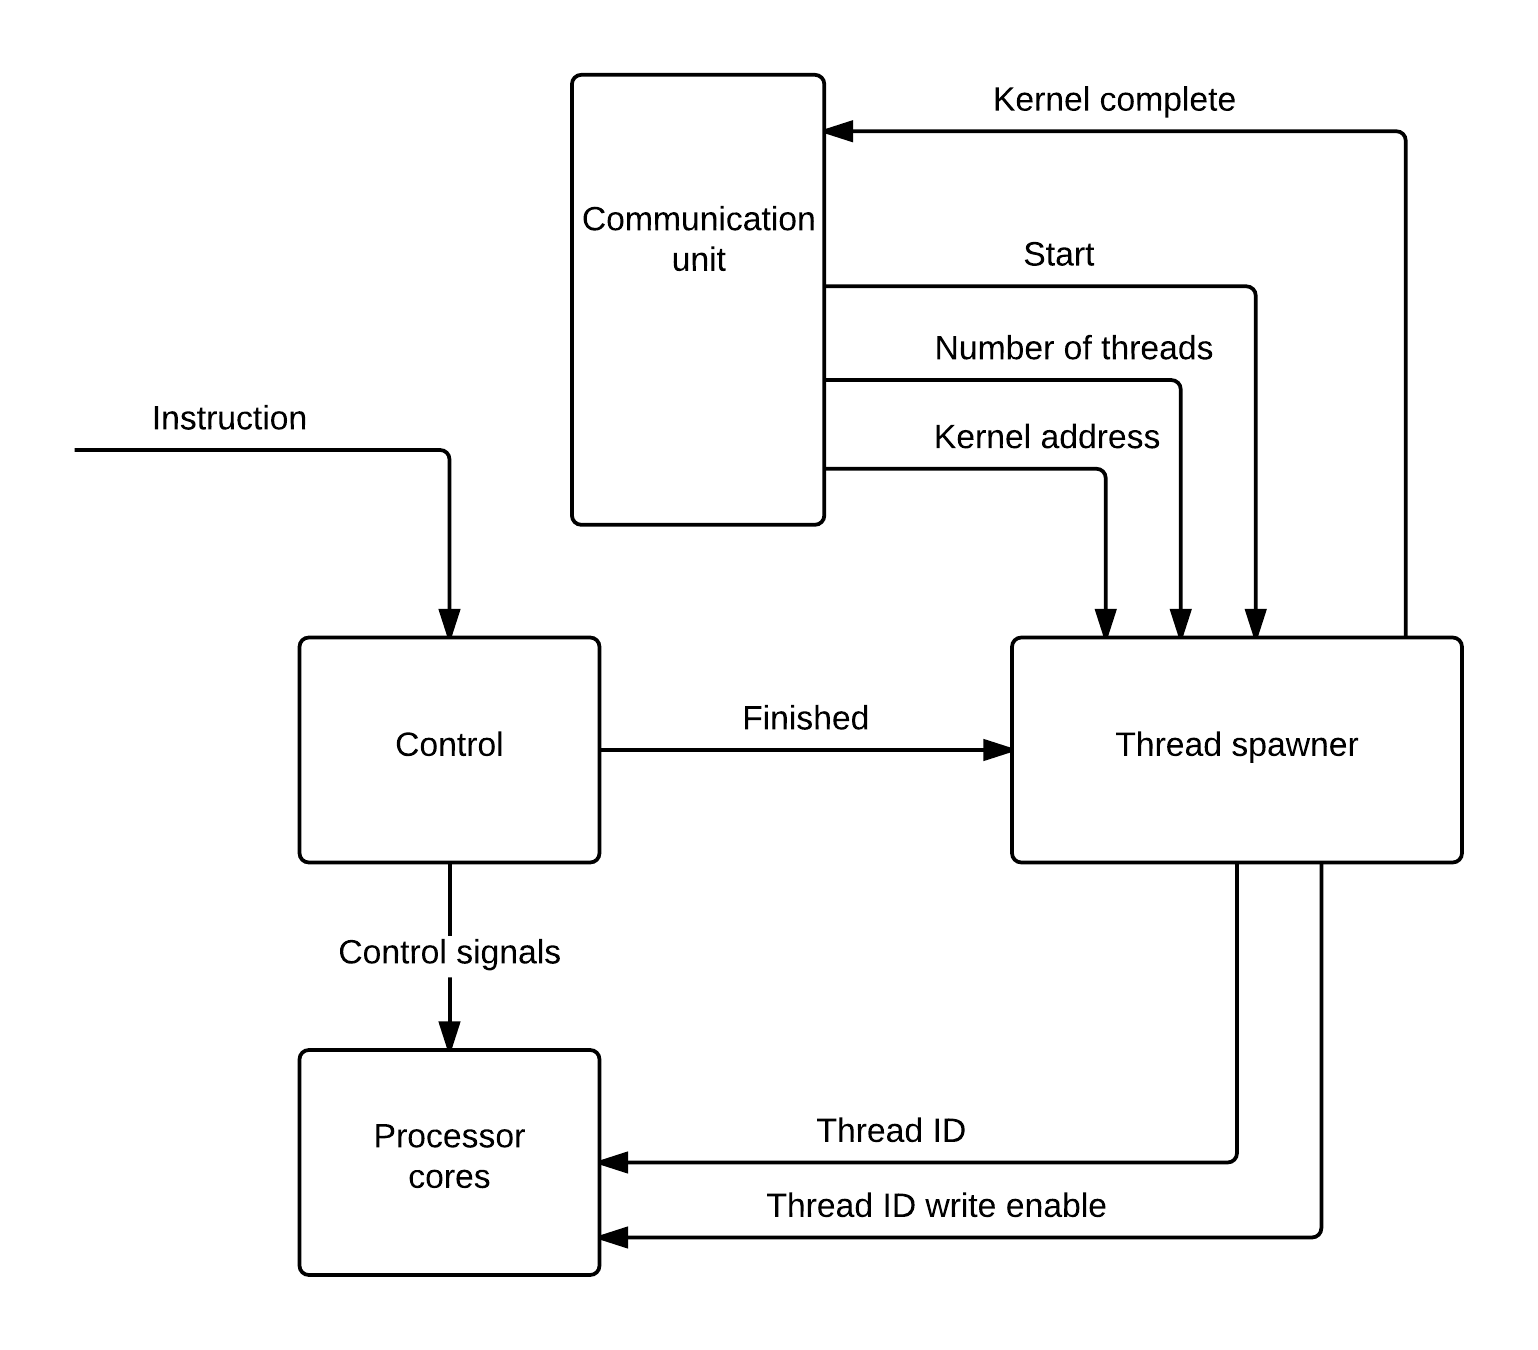
\includegraphics[width=1.1\textwidth]{../gpu/diagrams/thread_spawner_overview.png}
	\caption{Thread spawner and neighboring components.}
	\label{fig:thread_spawner_overview}
\end{figure}
\begin{figure}[H]
	\centering
	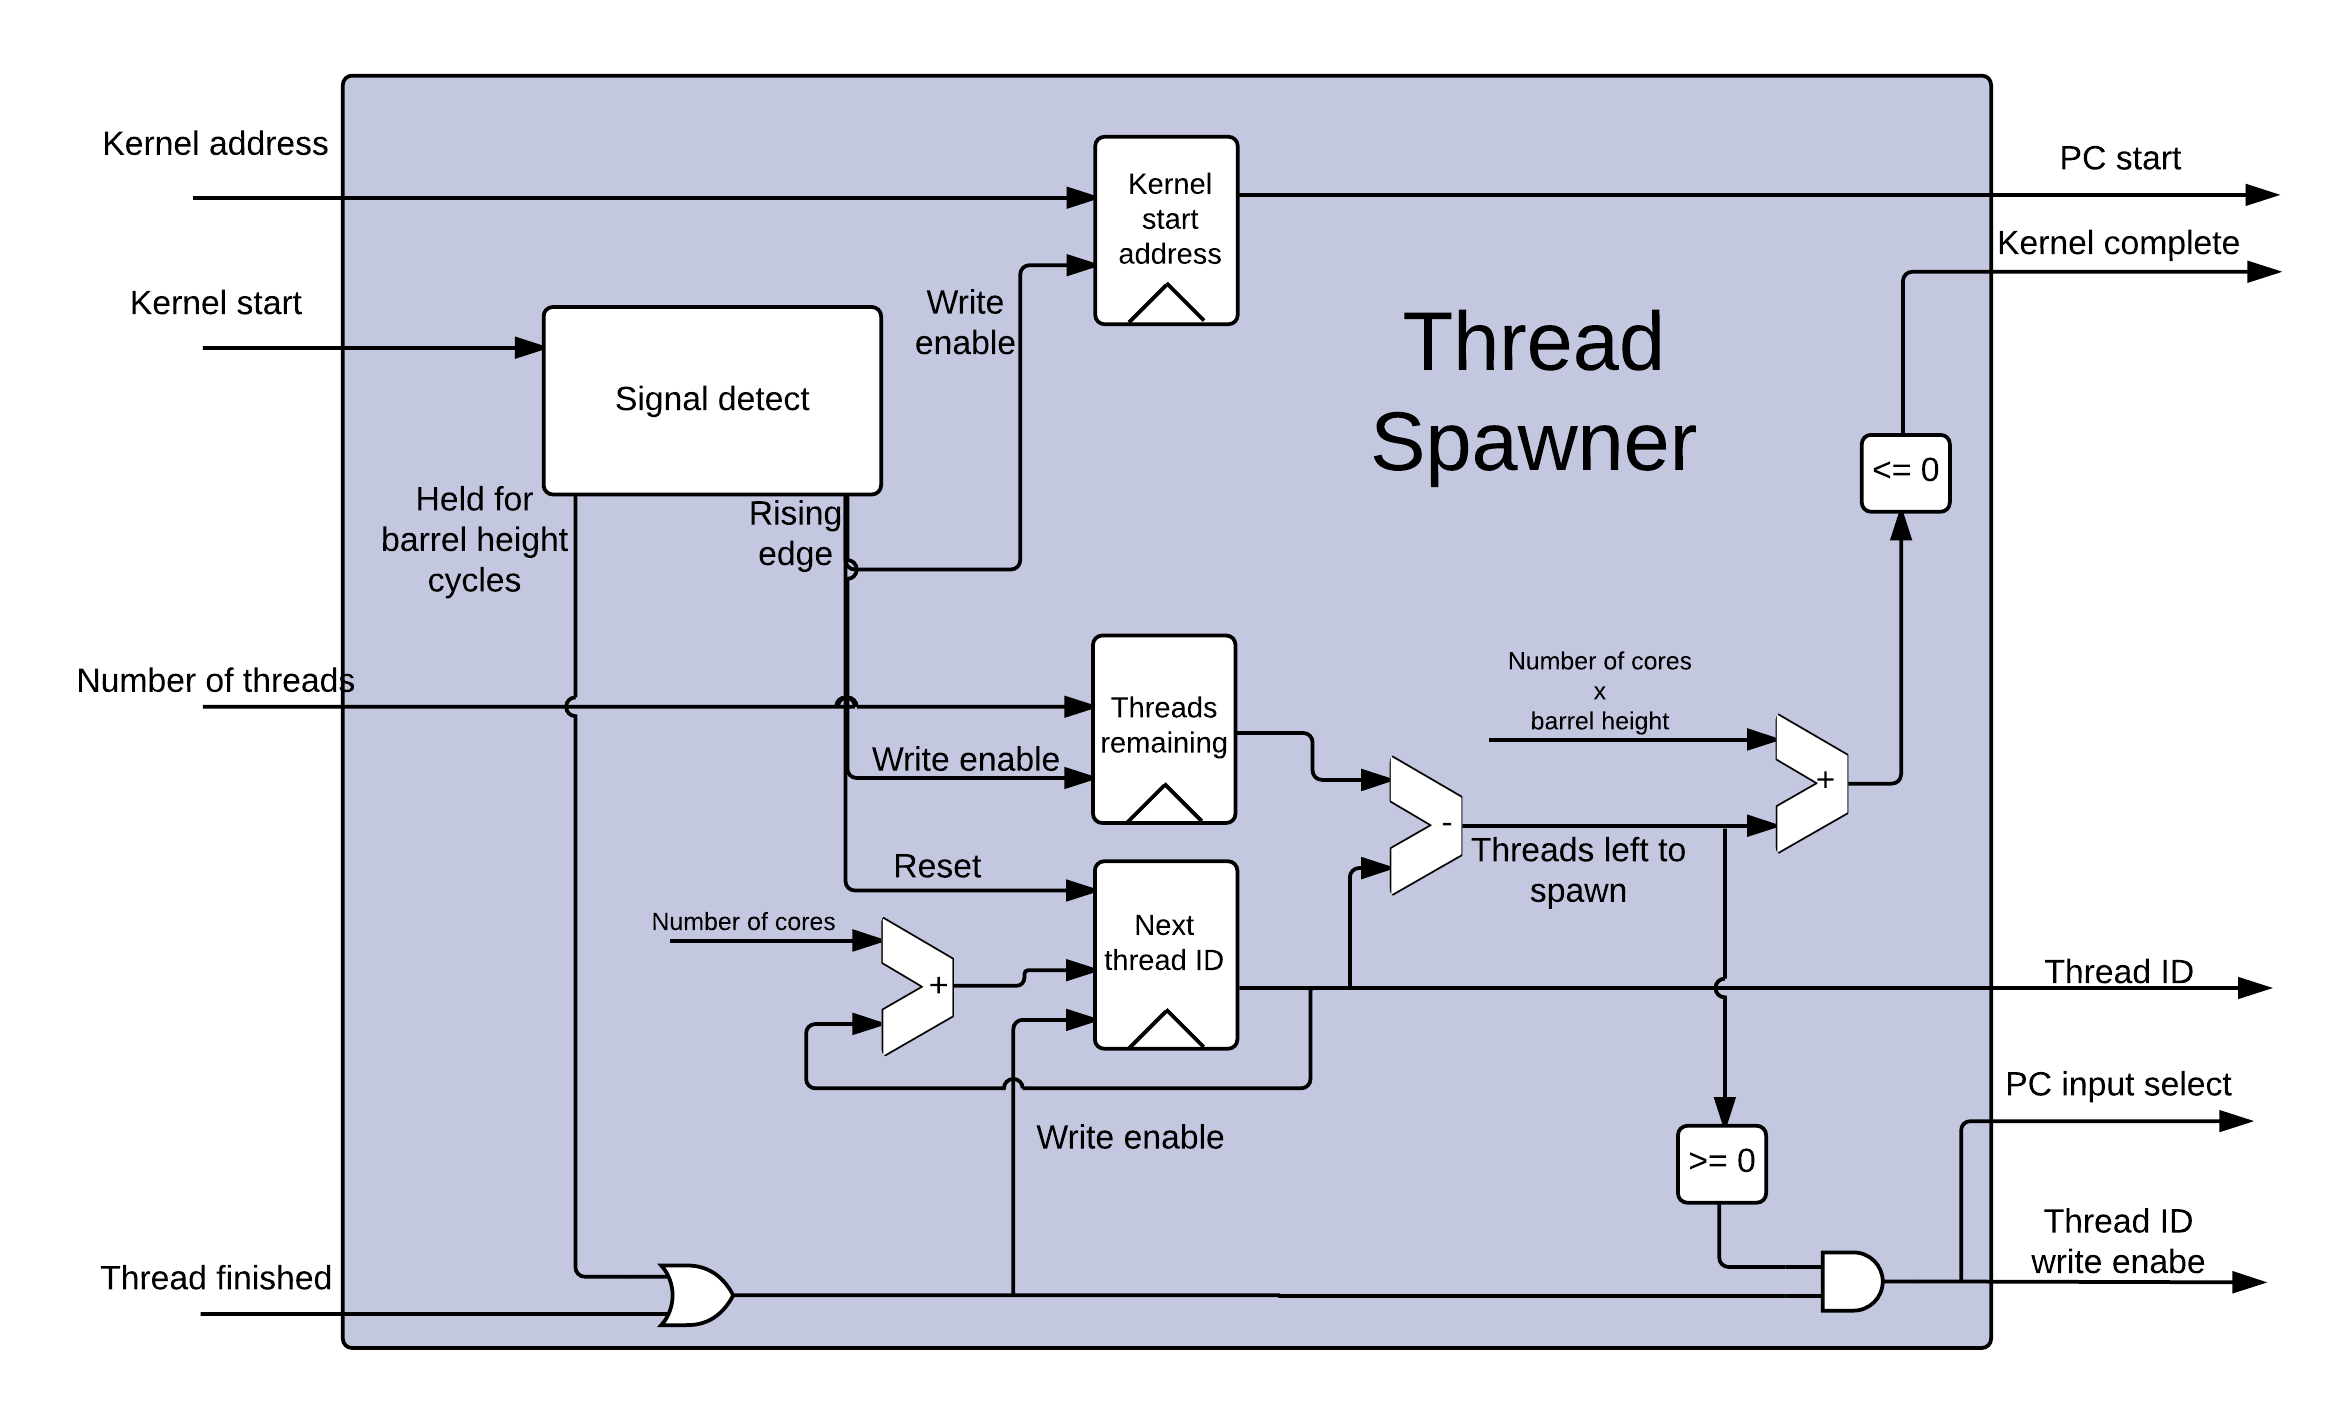
\includegraphics[width=1.1\textwidth]{../gpu/diagrams/thread_spawner.png}
	\caption{Thread spawner RTL implementation.}
	\label{fig:thread_spawner_rtl}
\end{figure}

The thread spawner is responsible for overseeing kernel execution.
It will spawn threads whenever necessary, handling thread setup and ensuring that the requested kernel is executed.
When all threads have finished executing, it will assert the kernel done signal, notifying the host program that computation has finished.

When a kernel invocation request is received, the thread spawner stores the provided base address of the kernel, the number of threads to spawn, and sets the next thread ID register to zero.
Threads are spawned one warp at a time into the currently active barrel line.
Therefore, on kernel start the thread spawner will spawn threads until the warp scheduler has made an entire rotation, or a barrel roll as we call it.

When a thread finishes execution, the control unit will assert the \emph{finished} signal to the thread spawner.
If there are threads left to spawn, the currently active barrel line will be filled with a new warp of threads.

But what does the spawning of a warp of threads actually entail?
All threads need a unique thread ID.
If the value of the next thread ID register is 4, and we have 4 processor cores,
core zero will write 4 to its thread ID register, core one 5, and so forth.
The next thread ID register is then incremented by the warp size, increasing it from 4 to 8.

